\documentclass{../../text-style}

\texttitle{Лекция 4: Работа с требованиями}

\begin{document}

\maketitle
\thispagestyle{empty}

\attribution{Тимофей Александрович Брыксин, бывш. доцент кафедры системного программирования СПбГУ}

\section{Что такое требования}

Требование --- это любое условие, которому должна соответствовать разрабатываемая система или программное средство. Требованием может быть часть функциональности, которой система должна обладать, или ограничение, которому система должна удовлетворять.

\section{Типы требований}

Требования к ПО состоят из нескольких уровней --- бизнес-требования, требования пользователей и функциональные требования. Вдобавок каждая система имеет свои нефункциональные требования.

\begin{center}
    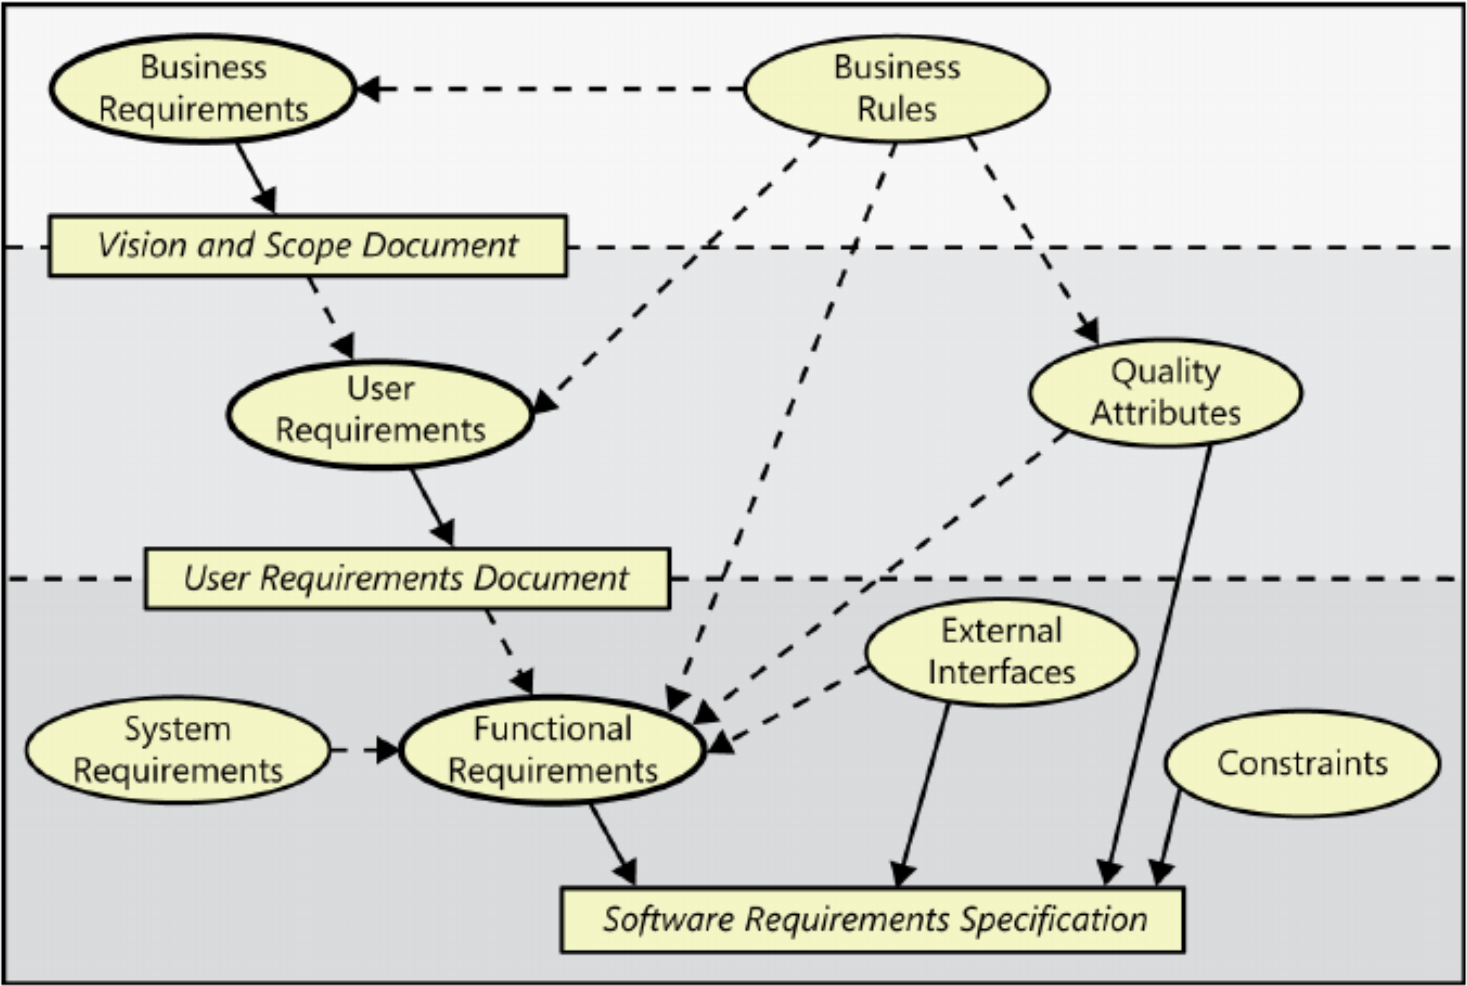
\includegraphics[width=0.9\textwidth]{requirements.png}
\end{center}


Бизнес-требования (business requirements) содержат высокоуровневые цели организации или заказчиков системы. Как правило, их высказывают те, кто финансируют проект, покупатели системы, менеджер реальных пользователей, отдел маркетинга и т.п. В этом документе объясняется, почему организации нужна такая система, то есть описаны цели, которые организация намерена достичь с её помощью.

Требования пользователей (user requirements) описывают цели и задачи, которые система позволит решить пользователям. К способам представления этого вида требований относятся варианты использования, сценарии и таблицы <<событие-отклик>>. Таким образом, в этом документе указано, что клиенты смогут делать с помощью системы.

Функциональные требования (functional requirements) определяют функциональность ПО, которую разработчики должны построить, чтобы пользователи смогли выполнить свои задачи в рамках бизнес-требований. Иногда именуемые требованиями поведения (behavioral requirements), они содержат положения с традиционным <<должен>> или <<должна>>: <<Система должна по электронной почте отправлять пользователю подтверждение о заказе>>. Функциональные требования описывают, что разработчику необходимо реализовать.

Бизнес-правила (business rules) включают корпоративные политики, правительственные постановления, промышленные стандарты и вычислительные алгоритмы. Бизнес-правила не являются требованиями к ПО, потому что они находятся снаружи границ любой системы ПО. Однако они часто налагают ограничения, определяя, кто может выполнять конкретные варианты использования, или диктовать, какими функциями должна обладать система, подчиняющаяся соответствующим правилам. Иногда бизнес-правила становятся источником атрибутов качества, которые реализуются в функциональности. В этом случае можно отследить происхождение конкретных функциональных требований вплоть до соответствующих им бизнес-правил.

Функциональные требования документируются в спецификации требований к ПО (software requirements specification, SRS), где описывается так полно, как необходимо, ожидаемое поведение системы. Спецификация может быть просто текстовым документом, базой данных или большой таблицей с требованиями, хранилищем данных в коммерческом инструменте управления требованиями или даже, может быть, просто кучей карточек для небольшого проекта. Спецификация требований к ПО используется при разработке, тестировании, обеспечении качества продукта, управлении проектом и связанных с проектом задачах.

В дополнение к функциональным требованиям спецификация содержит нефункциональные, где описаны цели и атрибуты качества. Атрибуты качества (quality attributes) представляют собой дополнительное описание функций продукта, выраженное через описание его характеристик, важных для пользователей или разработчиков. К таким характеристикам относятся легкость и простота использования, легкость перемещения, целостность, эффективность и устойчивость к сбоям. Другие нефункциональные требования описывают внешние взаимодействия между системой и внешним миром, а также ограничения дизайна и реализации. Ограничения (constraints) касаются выбора возможности разработки внешнего вида и структуры продукта.

Так, менеджеры и сотрудники отдела маркетинга определяют бизнес-требования для ПО, которые помогут их компании работать эффективнее (для информационных систем) или успешно конкурировать на рынке (для коммерческих продуктов). Каждое требование пользователя должно быть сопоставлено бизнес-требованию. На основе требований пользователя аналитики определяют функции, которые позволят пользователям выполнять их задачи. Разработчикам необходимы функциональные и нефункциональные требования, чтобы создавать решения с желаемой функциональностью, определенным качеством и требуемыми рабочими характеристиками, не выходя за рамки налагаемых ограничений.

Для примера рассмотрим программу подготовки текстов. Бизнес-требование может выглядеть так: <<Продукт позволит пользователям эффективно исправлять орфографические ошибки в тексте>>. Соответствующие требования пользователей могут содержать задачи (варианты использования) вроде такой: <<Найти орфографическую ошибку>> или <<Добавить слово в общий словарь>>. Проверка грамматики имеет множество индивидуальных функциональных требований, которые связаны с такими операциями, как поиск и выделение слова с ошибкой, отображение диалогового окна с фрагментом текста, где это слово находится, и замена слова с ошибкой корректным вариантом по всему тексту. Атрибут качества <<легкость и простота использования>> (usability) заявляется как важный посредством слова <<эффективно>> в бизнес-требованиях.

\section{Основные риски, связанные с требованиями}

\textbf{Недостаточное вовлечение пользователей.} Заказчики зачастую не понимают, почему так важно тщательно собрать требования и обеспечить их качество. Разработчики не всегда придают значение вовлечению пользователей в процесс из-за того, что среди них больше фанатов написания кода, чем любителей возиться с клиентами. Или же потому, что они считают, что всё уже знают о потребностях пользователей. В любом случае трудно добраться до людей, которые непосредственно будут иметь дело с продуктом, а те, кто выражает мнение пользователей, не всегда понимают, что тем нужно в реальности. Недостаточное вовлечение пользователей ведет к обнаружению ошибок в требованиях на поздних стадиях проекта, а значит, к задержке завершения проекта. Непосредственное и полноценное сотрудничество разработчиков с реальными пользователями на протяжении всего проекта очень сложно чем-то заменить.

\textbf{Игнорирование классов пользователей.} Большинство продуктов предназначены для нескольких групп пользователей, которые могут применять различные наборы функций с разной частотой и имеют опыт работы с ПО самого широкого диапазона. Если вы не определили важные классы пользователей для вашего продукта заранее, некоторые потребности клиентов могут быть не учтены. После идентификации всех классов удостоверьтесь, что по каждому из них у вас есть нужная информация.

\textbf{Разрастание требований пользователей.} Первоначально принятые планы не всегда основаны на реалистичном понимании размера и сложности требований, жесткая <<заморозка>> требований при этом не всегда возможна, а бездумное добавление требований в проект по ходу его развития может повлечь за собой серьёзные проблемы. Эти проблемы частично кроются в частых запросах пользователей на изменения, а частично в том, какими способами разработчики отвечают на них.

Чтобы управлять границами требований, для начала уточните бизнес-цели проекта, его рамки, ограничения, критерии успеха и ожидаемую пользу. Оцените, как предполагаемые характеристики или изменения требований отразятся на связанной с ними структуре. Эффективный процесс модификации заставляет интенсивнее работать аналитиков, которые помогут всем заинтересованным лицам принять обдуманные бизнес-решения относительно того, какие изменения следует принять, и увязать их стоимость со временем, ресурсами или возможными компромиссами. Изменения зачастую критически важны для успеха, однако они всегда имеют цену.

По мере того, как продукт модифицируется в процессе разработки, его архитектура может медленно разрушаться. Вставляемые в код неаккуратные быстрые правки (<<костыли>>) затрудняют понимание и поддержку продукта. Чтобы минимизировать возможность потери качества продукта в результате проблем такого рода, вначале продумайте (или даже протестируйте по возможности), как возможные изменения отразятся на архитектуре и дизайне, а уж затем реализуйте их непосредственно в коде.

\textbf{Двусмысленность требований} --- страшилка любой спецификации требований. Один из ее симптомов --- пользователь имеет возможность интерпретировать одно и то же положение по-разному. Другой --- что у нескольких читателей требований возникает разное представление о продукте. Кроме того, двусмысленность зачастую проистекает из неточности и плохой детализации требований, в результате чего разработчикам приходится заполнять возникающие пробелы собственными силами.

Двусмысленность ведет и к формированию различных ожиданий у заинтересованных лиц. Впоследствии некоторые из них удивляются, что же такое у нас получилось. Разработчики же впустую тратят время, занимаясь не теми проблемами, а тестировщики готовятся к проверке не тех особенностей поведения системы.

Один из способов обнаруживать двусмысленности --- пригласить различных представителей пользователей для официальной экспертизы требований. Пусть они просмотрят документ и выскажут свои замечания. Если они интерпретируют требования различными способами, то пусть неясность лучше проявится сейчас, а не гораздо позже, когда исправлять её будет сильно дороже. Другой способ вскрыть двусмысленность --- написать вариант тестирования для требования или построить прототип.

\textbf{Излишняя дополнительная функциональность.} Под этим пунктом понимают такие ситуации, когда разработчики добавляют функции, которых нет в спецификации, но им кажется, что это понравится пользователям. Зачастую же клиентам не нужны такие избыточные возможности, получается, что время, отведенное на реализацию, тратится впустую. Прежде чем просто вставлять новые функции, разработчики и аналитики должны представить свои творческие идеи на суд заказчиков. Задача команды --- чётко соблюдать требования спецификации, а не действовать за спиной клиентов без одобрения.

Другая сторона проблемы --- пользователи иногда требуют функции или элементы интерфейса, которые выглядят отлично, но не представляют особой ценности для продукта. Всё, что вы захотите добавить, стоит времени и денег, поэтому постарайтесь осознать ценность своевременного выпуска продукта. Чтобы избежать такой ситуации, отслеживайте каждый кусок функциональности до его первоисточника, чтобы четко понимать, почему именно он включен в продукт. Применение вариантов использования для извлечения требований поможет сосредоточиться на выборе тех элементов, которые помогут пользователям выполнять их бизнес-задачи.

\textbf{Урезанная спецификация.} Иногда сотрудников отдела маркетинга или менеджеров охватывает искушение создать урезанный вариант спецификации. Они ожидают, что разработчики <<нарастят мясо>> на основе этих набросков, пока проект развивается. Это годится для тесно сплочённой команды, которая занимается небольшой системой, или когда выполняется проект-исследование, или когда требования действительно гибкие. Хотя в большинстве случаев это всё-таки раздражает разработчиков (которые могут действовать при некорректных предположениях и с ограниченными инструкциями) и дезориентирует клиентов (которые не получат тот продукт, который они воображали).

\textbf{Небрежное планирование.} Когда к вам подбегает менеджер и говорит <<Я кое-что придумал для нового продукта. Когда вы сможете это сделать?>>, не отвечайте на подобный вопрос, пока больше не узнаете о проблеме. Неопределенные, недетализированные требования порождают слишком оптимистические оценки, за которыми часто следует перерасход времени и денег. При плохо просчитанной смете проект больше всего страдает из-за затрат на частые изменения требований, пропущенных требований, недостаточного взаимодействия с пользователями, недетализированной спецификации требований и плохого анализа. Когда вы высказываете оценку, то указывайте лучше временные рамки: лучший вариант, наиболее вероятный и худший вариант (хотя это в жизни на самом деле тоже не помогает, об оценках мы будем говорить в курсе дальше).

\section{Характеристики хороших требований}
Хорошее требование должно обладать следующими характеристиками:

\begin{itemize}
    \item Единичность --- требование описывает одну и только одну вещь.
    \item Завершенность --- требование полностью определено в одном месте и вся необходимая информация присутствует.
    \item Непротиворечивость --- требование не противоречит другим требованиям и полностью соответствует документации.
    \item Атомарность --- требование нельзя разделить на более мелкие.
    \item Отслеживаемость --- требование полностью или частично соответствует деловым нуждам как заявлено заинтересованными лицами и это чётко задокументировано.
    \item Актуальность --- требование не стало устаревшим с течением времени.
    \item Выполнимость --- требование может быть реализовано в рамках проекта.
    \item Недвусмысленность --- требование определено без обращения к техническому жаргону, акронимам и другим скрытым формулировкам. Оно выражает объекты и факты, а не субъективные мнения. Возможна одна и только одна его интерпретация. Определение не содержит нечетких фраз, использование отрицательных и составных утверждений запрещено.
    \item Обязательность --- требование представляет собой определенную заинтересованным лицом характеристику, отсутствие которой ведет к неполноценности решения, которая не может быть проигнорирована. Необязательное требование --- противоречие самому понятию требования.
    \item Проверяемость --- реализованность требования может быть проверена.
\end{itemize}

\section{Работа с требованиями}

Работа с требованиями --- процесс, включающий идентификацию, выявление, документацию, анализ, отслеживание, приоритизацию требований, достижение соглашений по требованиям и затем управление изменениями и уведомление заинтересованных лиц. Это непрерывный процесс на протяжении всего жизненного цикла продукта. В англоязычной среде также говорят о дисциплине <<инженерия требований>> (англ. Requirements Engineering). В процессе сбора требований важно принимать во внимание возможные противоречия требований различных заинтересованных лиц, таких как заказчики, разработчики или пользователи. Полнота и качество анализа требований играют ключевую роль в успехе всего проекта. А грамотное управление требованиями позволяет проекту избегать деградации при изменении требований в ходе разработки.

\section{Выявление требований}

Ранее мы обсуждали разные типы требований. Они собираются из разных источников на различных этапах работы над проектом, имеют различные цели и аудиторию и должны документироваться по-разному. Бизнес-требования не должны отменять каких-либо значительных пользовательских требований, кроме того, необходимо проследить, как из конкретных требований пользователей проистекают все функциональные требования. Также следует выявить нефункциональные характеристики, например предполагаемые качество и производительность. Рассмотрим основные моменты, про которые стоит помнить на этом этапе.

\textbf{Определение процесса формулирования требований.} Задокументируйте этапы выявления, анализа, определения и проверки требований. Наличие инструкций по выполнению ключевых операций поможет аналитикам качественно и согласованно выполнить их работу. Кроме того, вам будет проще поставить задачи по созданию требований и графики, а также продумать необходимые ресурсы.

\textbf{Определение классов пользователей и их характеристик.} Чтобы не упустить из виду потребности отдельных пользователей, выделите их в группы. Например, это можно сделать по частоте работы с ПО, используемым функциям, уровню привилегий или навыкам работы. Опишите основных персонажей: их обязанности, необходимости, пожелания, личные характеристики и т.п. --- всё, что способно повлиять на архитектуру продукта.

\textbf{Выбор типичного пользователя в каждом классе пользователей.} Очень здорово, если в каждой группе пользователей можно выделить человека, который сможет точно передавать настроения и нужды остальных в этой группе. Он представляет потребности определенного класса пользователей и принимает решения от их лица. В случае, когда все пользователи ваши коллеги, такого человека выбрать проще. При коммерческой разработке расспросите клиентов или используйте площадки бета-тестирования. Выбранные вами люди должны принимать постоянное участие в проекте и обладать полномочиями для принятия решений, касающихся пользовательских требований. Но нужно соблюдать осторожность и не позволять этому человеку выдавать собственные пожелания за требования всей группы.

\textbf{Создание фокус-групп и проведение интервью с типичными пользователями.} Фокус-группы особенно значимы при разработке коммерческих продуктов, когда приходится иметь дело с большой и разнородной клиентской базой. У фокус-групп обычно нет полномочий на принятие решений, однако мнение людей послушать полезно. С представителями групп пользователей можно провести персональные интервью.

\textbf{Наблюдение за пользователями на рабочих местах.} Наблюдая за работой пользователей, можно собрать много информации о контексте потенциального применения нового продукта. Простые диаграммы рабочих потоков, а также диаграммы потоков данных позволяют выяснить, где, как и какие данные задействовал пользователь. Документируя ход бизнес-процесса, удается определить требования к системе, предназначенной для поддержки этого процесса. Иногда даже выясняется, что для выполнения деловых задач клиентам вовсе и не требуется новое ПО.

Примером диаграммы, с помощью которой можно фиксировать рабочие процессы, является диаграмма потока данных, представленная ниже. 

\begin{center}
    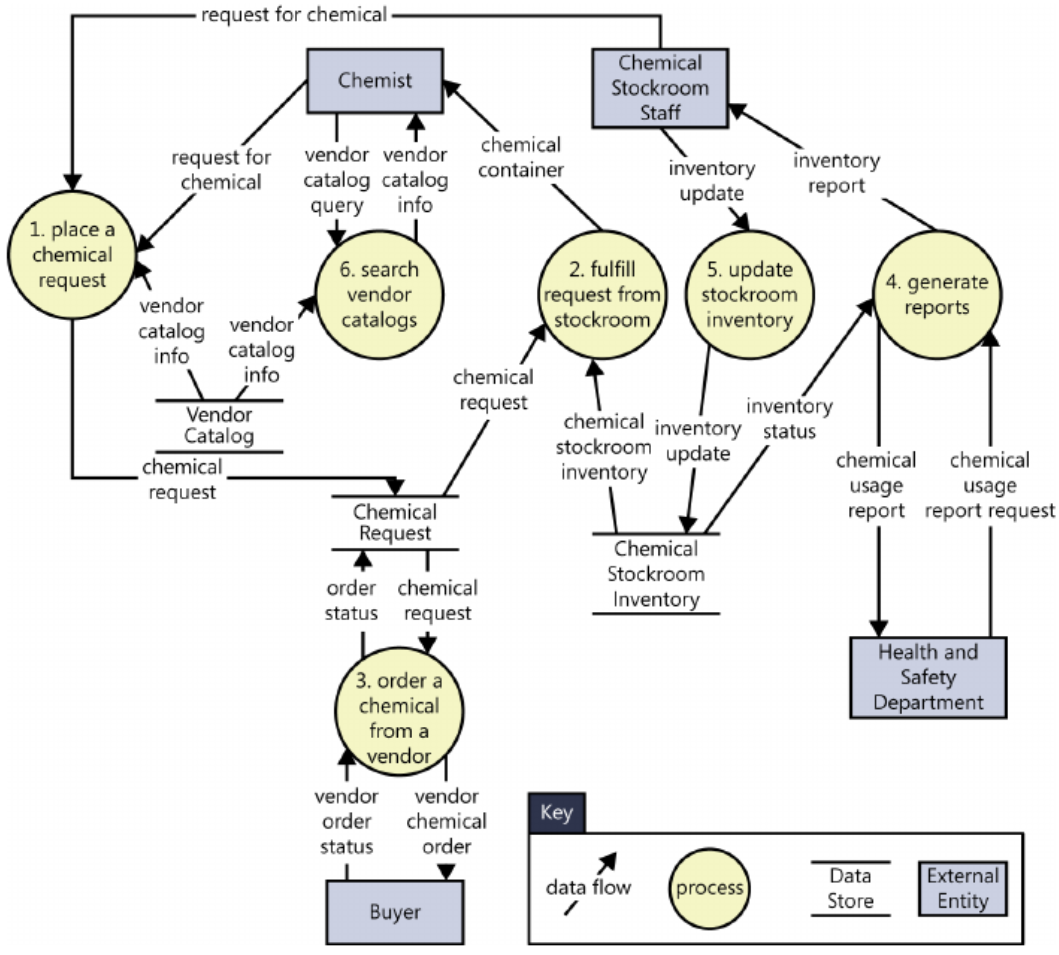
\includegraphics[width=0.9\textwidth]{dfd.png}
\end{center}

\textbf{Изучение отчетов о проблемах работающих систем с целью поиска новых идей.} Поступающие от клиентов отчеты о проблемах и предложения о расширении функциональности --- отличный источник идей о возможностях, которые можно реализовать в следующей версии или новом продукте. Этой информации обычно бывает в избытке у сотрудников службы поддержки. Также можно проанализировать багтрекер и другие похожие системы.

\textbf{Определение системных событий и реакции на них.} Определите возможные внешние события и ожидаемую реакцию системы на них. Это могут быть сигналы и данные, получаемые от внешнего оборудования, а также временные события, вызывающие ответную реакцию, например ежедневная передача данных, генерируемых системой, внешнему объекту. В бизнес-приложениях бизнес-события напрямую связаны с задачами.

\textbf{Создание документа об образе и границах проекта.} Документ об образе и границах проекта содержит бизнес-требования к продукту. Описание образа проекта позволит всем заинтересованным лицам в общих чертах понять назначение продукта. Границы проекта определяют, что следует реализовать в первых версиях продукта. Образ и границы проекта --- хорошая база для оценки предлагаемых требований. Образ продукта должен оставаться от версии к версии относительно стабильным, но для каждой глобальной версии необходимо составлять отдельный документ о границах.

\section{Анализ требований}

Анализ требований подразумевает их детализацию, гарантирующую, что требования понимают все заинтересованные лица, а также тщательное исследование требований на предмет ошибок, пробелов и других недостатков. Кроме того, анализ включает создание прототипов, анализ осуществимости и согласование приоритетов. Цель анализа --- достаточно качественно и подробно описать требования, позволяющие менеджерам реалистично оценить все затраты на проект, а техническому персоналу --- начать проектирование, сборку и тестирование.

Зачастую отдельные требования стоит представить несколькими способами, например в текстовой и графической форме. Это позволит выявить их особенности и проблемы, не заметные при представлении одним способом. Также это помогает всем заинтересованным лицам выработать согласованное представление об итогах разработки продукта. 

Рассмотрим основные виды деятельности на этом этапе.

\textbf{Анализ осуществимости требований.} Проанализируйте, насколько реально реализовать каждое требование при разумных затратах и с приемлемой производительностью в предполагаемой среде. Рассмотрите риски, связанные с реализацией каждого требования, включая конфликты с другими требованиями, зависимость от внешних факторов и препятствия технического характера.

\textbf{Определение приоритетов требований.} Определите относительные приоритеты реализации функций продукта, решаемых задач или отдельных требований. На основании приоритетов установите, в какой версии будет реализована та или иная функция или набор требований. Подтверждая изменения, распределите все их по конкретным версиям и включите в план выпуска этих версий затраты, необходимые на внесение изменений. В ходе работы над проектом стоит периодически переоценивать и корректировать приоритеты в соответствии с потребностями клиента, условиями рынка и бизнес-целями.

\textbf{Моделирование требований.} В отличие от подробной информации, представленной в спецификации требований к ПО или пользовательского интерфейса прототипа, графическая модель анализа отображает требования на высоком уровне абстракции. Модели позволяют выявить некорректные, несогласованные, отсутствующие и избыточные требования. К таким моделям относятся диаграммы потоков данных, диаграммы <<сущность-связь>>, диаграммы конечных автоматов, карты экранов, диаграммы классов, диаграммы последовательностей, диаграммы взаимодействий, таблицы и деревья решений и многое другое.

\textbf{Создание словаря терминов.} В этом документе соберите определения всех элементов и структур данных, связанных с системой, что позволяет всем участникам проекта использовать согласованные определения данных. На стадии работы над требованиями словарь должен содержать определения элементов данных, относящихся к предметной области, чтобы клиентам и разработчикам было проще общаться. 

\textbf{Создание контекстной диаграммы.} Контекстная диаграмма --- простая модель анализа, отображающая место новой системы в соответствующей среде. Она определяет границы и интерфейсы между разрабатываемой системой и сущностями, внешними для этой системы, например пользователями, устройствами и прочими информационными системами. 

\begin{center}
    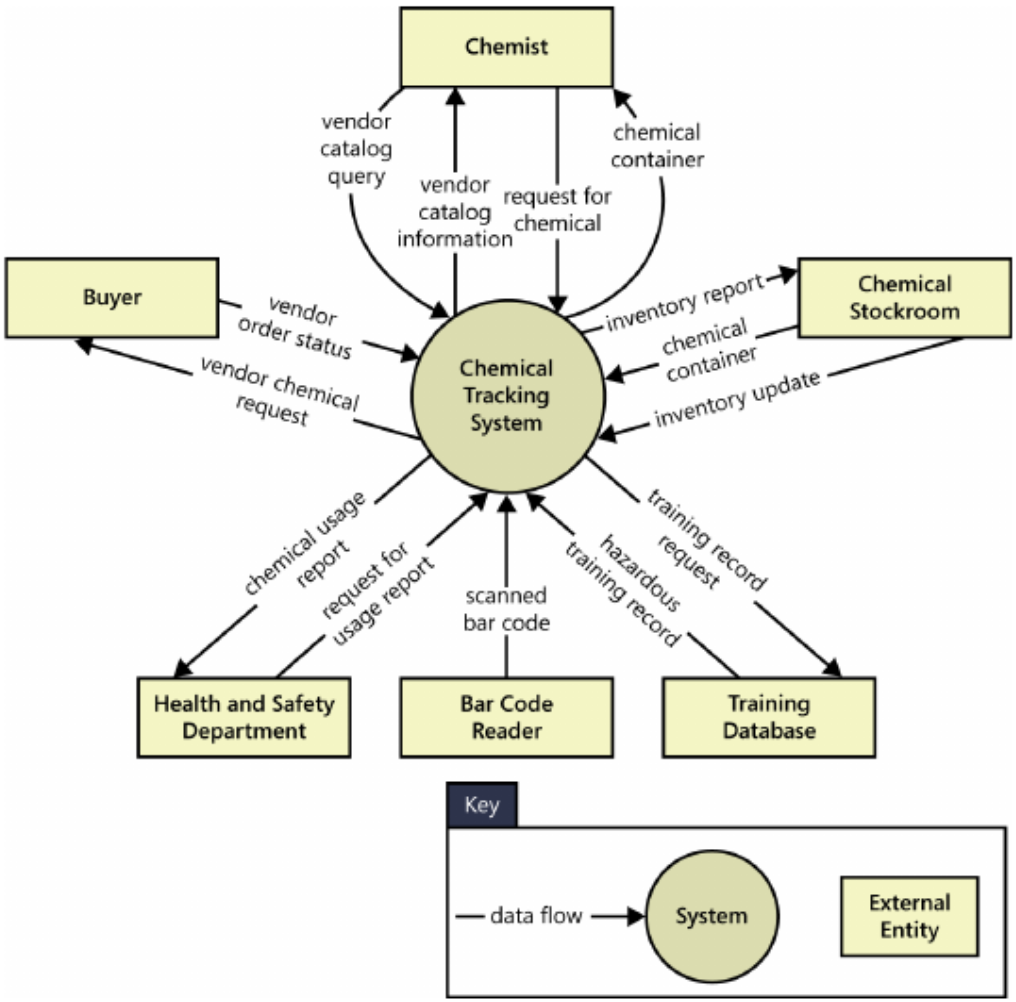
\includegraphics[width=0.8\textwidth]{contextDiagram.png}
\end{center}

\textbf{Создание пользовательского интерфейса и технических прототипов.} Если разработчики или пользователи не совсем уверены насчет требований, создайте прототип --- частичную, возможную или предварительную версию продукта, которая сделает концепции и возможности более осязаемыми. Оценка прототипа поможет всем заинтересованным лицам достичь взаимопонимания по решаемой проблеме.

\section{Проверка требований}

Процесс проверки гарантирует, что все положения требований корректны, отражают желаемые качественные характеристики и удовлетворяют потребностям клиента. Может оказаться, что требования, в спецификации требований к ПО выглядевшие превосходно, при реализации чреваты проблемами. В большинстве случаев удается выявить двусмысленности и неопределенности, написав для требований сценарии тестирования. Так как в большинстве случаев требования должны стать надежной основой для проектирования и итоговой проверки системы посредством системного тестирования или тестирования на приемлемость для пользователей, эти проблемы необходимо устранить.

\textbf{Изучение документов с требованиями.} Официальная проверка документирования требований --- один из наиболее ценных способов проверки качества ПО. Соберите небольшую команду, члены которой представляют различные направления (например, аналитик, клиент, разработчик и специалист по тестированию), и тщательно изучите спецификацию требований к ПО, модель анализа и соответствующую информацию на предмет недостатков. Также полезно провести в ходе формулирования требований их неофициальный предварительный просмотр. И хотя реализовать это на практике непросто, данный прием --- один из самых ценных.

\textbf{Определение критериев приемлемости.} Предложите пользователям описать, как они собираются определять соответствие продукта их потребностям и его пригодность к работе.

\textbf{Тестирование требований.} На основе пользовательских требований создайте сценарии функционального тестирования и задокументируйте ожидаемое поведение продукта в конкретных условиях. Совместно с клиентами изучите сценарии тестирования и убедитесь, что они отражают нужное поведение системы. Проследите связь сценариев тестирования с функциональными требованиями и удостоверьтесь, что ни одно требование не пропущено и что для всех требований есть соответствующие сценарии тестирования. Если используемые формализмы позволяют, запустите сценарии, чтобы удостовериться в правильности моделей анализа и прототипов.

\section{Процесс работы с требованиями}

Не ждите, что все действия по выявлению, анализу, спецификации и проверке требований удастся выполнить последовательно и за один проход. На практике эти действия выполняются попеременно, поэтапно и повторяются.

\begin{center}
    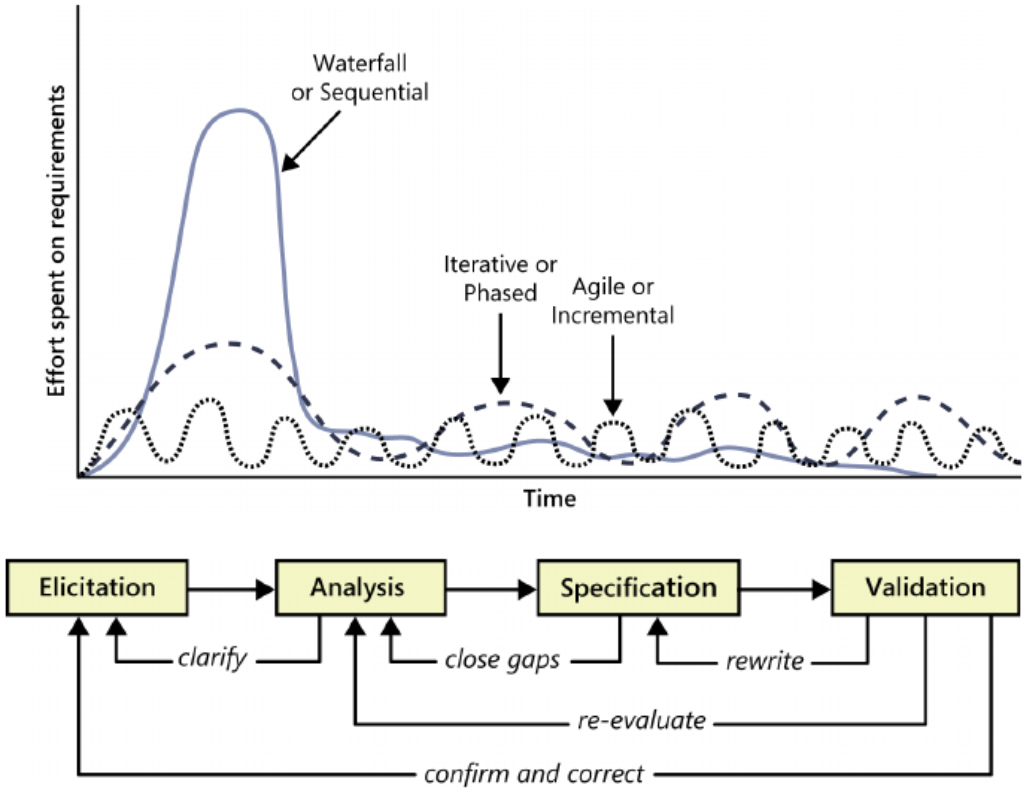
\includegraphics[width=0.9\textwidth]{requirementsProcess2.png}
\end{center}

Работая с клиентами, аналитики будут задавать вопросы, выслушивать ответы и наблюдать за действиями клиентов (выявление требований). Далее полученная информация обрабатывается, классифицируется по различным категориям и соотносится с потребностями клиентов (анализ). Затем информация от клиентов и выработанные требования оформляются в виде письменных документов и диаграмм (спецификация), представителям пользователей предлагается подтвердить, что написанный текст точен и полон, и исправить возможные ошибки (проверка). Этот итерационный процесс и есть процедура создания требований.

\section{Навыки, необходимые аналитику}

Чтобы быть хорошим аналитиком, нужна соответствующая подготовка. Аналитик должен уметь применять разные средства сбора информации и представлять эту информацию различными способами на нормальном и понятном языке. Профессионал в этой области обладает одновременно развитыми коммуникационными навыками, знанием психологии межличностного общения, техническими знаниями, знаниями предметной области бизнеса и личными качествами, подходящими для этой работы. Основные факторы успеха --- терпение и искреннее желание работать с людьми, но не менее важны и навыки, описанные далее.

\textbf{Умение задавать вопросы.} Большая часть информации о требованиях извлекается в ходе беседы с людьми, и поэтому аналитик должен уметь общаться с разными людьми и группами, только так ему удастся выявить их потребности. При этом работать со старшими менеджерами или чрезмерно самоуверенными или агрессивными людьми будет трудно. Для выяснения существенных требований пользователей необходимо задавать правильные вопросы. Например, пользователи обычно делают акцент на ожидаемом поведении системы. Тем не менее значительная часть кода будет обрабатывать исключения, поэтому вам следует определить возможные условия ошибок и реакцию системы на них. Нужно научиться задавать вопросы, которые раскрывают и проясняют неопределенности, расхождения во мнениях, предположения и невысказанные ожидания пользователей.

\textbf{Умение слушать.} Чтобы стать специалистом, надо научиться эффективно слушать. Активное слушание подразумевает устранение помех, сохранение вежливой позы и зрительный контакт, а также повторение основных моментов для закрепления их понимания. Нужно уметь моментально схватывать, что говорят люди, и уметь читать между строк, чтобы обнаружить вещи, о которых они стесняются говорить. Избегайте налагать собственный фильтр понимания на высказывания клиентов, но при этом ищите допущения, которые подчеркивали бы мысли других или их интерпретацию.

\textbf{Умение наблюдать.} Внимательный аналитик запомнит высказанные мимоходом комментарии, которые могут оказаться важными. Наблюдая за тем, как пользователь выполняет свои обязанности или работает с имеющимся приложением, опытный аналитик выявит моменты, о которых пользователь даже не упомянул. Наблюдательность иногда помогает направить дискуссию в новое русло, чтобы выявить дополнительные требования, о которых никто ничего не сказал.

\textbf{Навыки межличностного общения.} Аналитик должен уметь организовать людей с разными интересами для совместной работы, и уверенно чувствовать себя в разговорах с сотрудниками, занимающими разные должности в организации. Подумайте, как сложно иметь дело с сотрудниками из виртуальных групп, различающихся по географическому, временному, культурному или языковому признаку.

\textbf{Навыки анализа.} Эффективный аналитик способен думать на нескольких уровнях абстракции. Иногда требуется перейти от сведений высшего порядка к подробностям. В некоторых случаях на основе потребности одного из пользователей сформулировать набор требований, которые удовлетворят большинство пользователей данного класса. Критически оценивайте информацию, полученную на основе разных источников, чтобы урегулировать конфликты, отделить мимолетные желания пользователей от их реальных потребностей и отличать варианты решений от требований.

\textbf{Навыки написания документации.} Основной итог процесса создания требований --- письменная спецификация с информацией для клиентов, отдела маркетинга и технического персонала. Аналитик должен отлично владеть языком и ясно выражать сложные идеи.

\textbf{Навыки моделирования.} Аналитик должен уметь работать с разнообразными средствами, начиная с древних блок-схем и структурированных моделей анализа (диаграммы потоков информации, диаграммы <<сущность-связь>> и т.д.) и заканчивая современным языком UML. Некоторые из этих средств полезны при общении с пользователями, другие --- с разработчиками. Аналитику следует объяснить другим участникам проекта ценность использования этих методов и то, как работать с их данными.

\textbf{Организационные навыки.} Аналитик имеет дело с большим объёмом беспорядочной информации, собранной на первом этапе. Чтобы справиться с данными и выстроить согласованное целое, вам потребуются исключительные организационные навыки, а также терпение и упорство для вычленения основных идей из хаоса.

\textbf{Творческий подход.} Аналитик --- не просто клерк, записывающий все высказывания клиентов. Лучшие аналитики изобретают требования. Они предлагают инновационные функции продуктов, новые рыночные возможности и возможности для бизнеса и думают, как удивить и удовлетворить своих клиентов. Отличный аналитик творчески подходит к делу: рассказывая о системе, ему удается удивить клиента -- тот даже не всегда подозревает, что такая функциональность возможна.

Для профессии системного аналитика также есть стандарты, поразглядывать один из них, например, можно тут: \url{https://systems.education/standards}.

\section{Создаваемые документы}

На этапе спецификации требований обычно создаются следующие документы:

\begin{itemize}
    \item документ об образе и границах системы,
    \item глоссарий,
    \item модель требований,
    \item прототип пользовательского интерфейса,
    \item спецификация требований.
\end{itemize}

Создавать их можно с разной степенью формальности или даже не создавать совсем, но наличие их может сильно помочь при дальнейшем ходе проекта. Глоссарий и прототипы пользовательских интерфейсов мы уже в некотором виде обсудили, поговорим про остальные документы.

\subsection{Документ об образе и границах системы}

Если у участников проекта разное представление о предполагаемых границах и целях проекта, то им трудно будет договориться о том, какое функциональное требование относится к спецификации требований, а какое не относится.

Проект, в котором нет четко определенного и согласованного направления, сложно довести до успешного завершения, поскольку никто не понимает, где оно. Участники проекта могут, сами того не осознавая, решать прямо противоположные задачи, если у них разные бизнес-цели и приоритеты. Четкое представление образа и границ проекта особенно важно при распределенной разработке ПО, когда географическое разделение участников замедляет ежедневное взаимодействие, упрощающее коллективную работу.

Проблемы, касающиеся образа и границ, необходимо разрешать до спецификации детализированных функциональных требований. Положение о рамках и ограничениях проекта необычайно полезно при обсуждении предлагаемых функций и целевых выпусков. Кроме того, на него можно ссылаться при принятии решений об изменении и расширении требований. В некоторых компаниях основные положения об образе и границах помещают на схему, которую приносят на каждое проектное совещание, чтобы все смогли быстро оценить, не выходит ли предложенное изменение за рамки проекта.

Образ или концепция продукта (product vision) выстраивает работу всех заинтересованных лиц в одном направлении. Он описывает, что продукт представляет собой сейчас и каким он станет впоследствии. Границы проекта (project scope) показывают, к какой области конечного долгосрочного образа продукта будет направлен текущий проект. В положении о границах определена черта между тем, что входит в проект и тем, что остается вовне. То есть указанные рамки также определяют ограничения проекта. 

Рассмотрим возможную структуру такого документа.

\begin{enumerate}
    \item \textbf{Бизнес-требования.} Проекты должны выпускаться с убеждением, что новый продукт для кого-то сделает мир лучше. Бизнес-требования описывают основные преимущества, которые новая система даст ее заказчикам, покупателям и пользователям.
    \begin{enumerate}
        \item \textbf{Исходные данные.} Этот раздел суммирует обоснование и содержание нового продукта. В него помещают общее описание предыстории или ситуации, в результате которых было принято решение о создании продукта.
        \item \textbf{Возможности бизнеса.} Для коммерческого продукта описывают существующие рыночные возможности и рынок, на котором продукту придется конкурировать с другими продуктами. Обычно здесь описывают бизнес-проблему, которая разрешается посредством этого продукта, или бизнес-процессы, для улучшения которых требуется продукт, а также среду, в которой система будет использоваться. Кроме того, сюда можно же добавить и сравнительную оценку существующих продуктов и возможных решений, указав, в чем заключается привлекательность продукта и его преимущества. Покажите, насколько он соответствует тенденциям рынка, развитию технологий или корпоративной стратегии.
        \item \textbf{Бизнес-цели и критерии успеха.} Данный раздел суммирует важные преимущества бизнеса, предоставляемые продуктом, в количественном и измеряемом виде. Здесь же нужно отметить, как заинтересованные лица будут определять и измерять успех проекта. Установите факторы, которые максимально влияют на успех проекта, и те, которые организация может контролировать, и те, которые находятся вне сферы ее влияния. Определите меру для оценки того, были ли достигнуты бизнес-цели.
        \item \textbf{Потребности клиентов или рынка.} Опишите потребности типичных покупателей или целевых сегментов рынка, включая потребности, которые не удовлетворяют настоящие продукты или информационные системы. Представьте проблемы, с которыми в настоящее время сталкиваются клиенты и которые решит новая система, и предоставьте примеры того, как покупатели будут использовать этот продукт. Определите на высоком уровне все известные важные требования к интерфейсу или производительности, но не касайтесь деталей дизайна или реализации.
        \item \textbf{Бизнес-риски.} Этот раздел обобщает важнейшие бизнес-риски, связанные с созданием этого продукта. В категории рисков входят рыночная конкуренция, временные факторы, приемлемость для пользователей, проблемы, связанные с реализацией, и возможные негативные факторы, влияющие на бизнес. Оцените возможные потери от каждого фактора риска, вероятность его возникновения и вашу способность контролировать его. Определите все возможные действия по смягчению ситуации.
    \end{enumerate}
    \item \textbf{Концепция (vision) решения.} В этом разделе документа определяется стратегический образ системы, позволяющей выполнять бизнес-задачи. Этот образ обеспечивает основу для принятия решений в течение жизненного цикла продукта. В него не надо включать детали функциональных требований или информацию, связанную с планированием проекта.
    \begin{enumerate}
        \item \textbf{Положение об образе проекта.} Составьте сжатое положение об образе проекта, обобщающее долгосрочные цели и назначение нового продукта. В этом документе следует отразить сбалансированный образ, удовлетворяющий различные заинтересованные лица. Он может быть несколько идеалистичным, но должен быть основан на существующих или предполагаемых рыночных факторах, архитектуре предприятия, стратегическом направлении развития компании или ограничениях ресурсов. Далее показан шаблон, состоящий из ключевых слов, который неплохо подходит для этого раздела:

        Для [целевая аудитория покупателей], которые [потребности или возможности пользователей], [имя продукта]  является [категория продукта], который [ключевое преимущество, основная причина для покупки или использования]. В отличие от [основной конкурирующий продукт, текущая система или текущий бизнес-процесс] наш продукт [основное отличие и преимущество нового продукта].
        \item \textbf{Основные функции.} Опишите каждую основную функцию нового продукта или возможность, предоставляемую пользователям, подчеркивая те из них, которые отличают его от предыдущих или конкурирующих продуктов. Дав каждой функции уникальное имя, вы сможете отследить каждую функцию до отдельных требований пользователей, функциональных требований и других элементов систем. Для наглядного отображения декомпозиции функций проекта часто удобно использовать следующую диаграмму:
        \begin{center}
            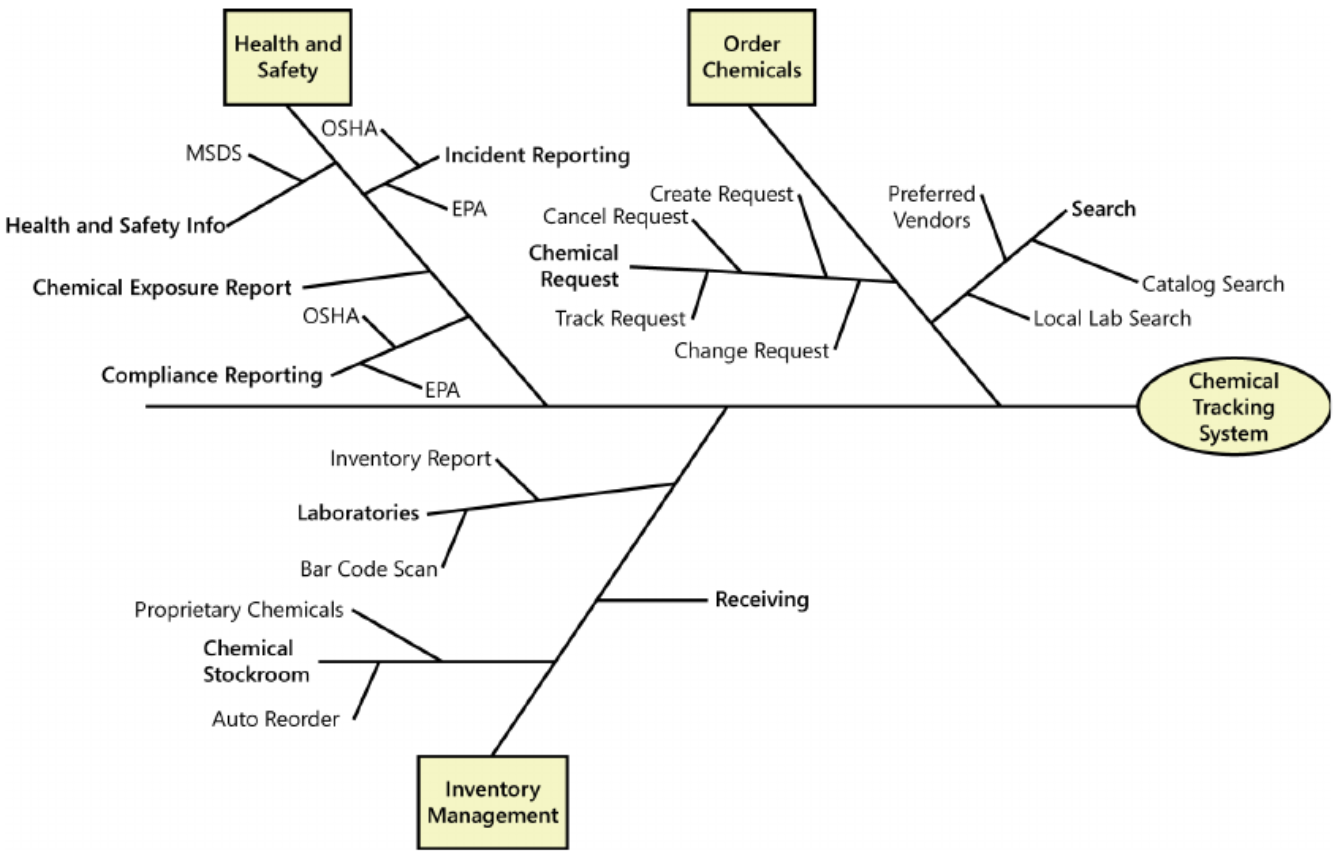
\includegraphics[width=0.8\textwidth]{featureTree.png}
        \end{center}

        Она отображает функции, организованные в иерархически устроенные логические группы. Обычно на таких диаграммах отображают не больше трёх уровней декомпозиции.
        \item \textbf{Предположения и зависимости.} Задокументируйте все предположения, сделанные заинтересованными лицами, когда они обдумывали проект и создавали данный документ об образе и границах. Часто предположения одних лиц не разделяют другие стороны. Если вы запишите их и просмотрите позже, то получите возможность обговорить основные положения проекта. Так вы избежите путаницы и ухудшения ситуации в будущем. Также задокументируйте важнейшие зависимости проекта от внешних факторов: изменения индустриальных стандартов или правительственных положений, других проектов, поставщиков со стороны или партнеров по разработке.
    \end{enumerate}
    \item \textbf{Масштабы и ограничения проекта.} В этом разделе необходимо указать, что может делать система, а что не может. Рамки и ограничения помогают установить реалистичные ожидания заинтересованных лиц. Иногда клиенты запрашивают функции, слишком дорогостоящие или выходящие за предполагаемые границы продукта. Требования, выходящие за границы продукта, следует отклонять, если только они не настолько ценны, чтобы специально под них расширить проект, естественно, соответствующим образом изменив в бюджет, график и кадровый состав. Документируйте отклоненные требования и причины отказа от них, поскольку они имеют свойство появляться снова.
    \begin{enumerate}
        \item \textbf{Объем первоначальной версии.} Обобщает основные запланированные функции, включенные в первоначальную версию продукта. Опишите характеристики качества, которые позволят продукту предоставлять предполагаемые выгоды различным классам пользователей. Если ваша задача --- сосредоточиться на разработке и уложиться в график, вам следует избегать искушения включить в версию 1.0 каждую функцию, которая когда-нибудь в будущем может понадобиться какому-то потенциальному покупателю.

        Увеличение сроков и сдвиг графика --- типичный исход такого расползания объема. Сосредоточьтесь на наиболее ценных функциях, имеющих максимально приемлемую стоимость, годных для самой широкой целевой аудитории, которые удастся создать как можно раньше. Версия 1.0 не обязательно должна быть супербыстрой, красиво оформленной или легкой в использовании, но она должна быть надежной. Первая версия системы выполняет лишь базовые задачи. В будущие выпуски будут включены дополнительные функции, возможности и средства, обеспечивающие легкость и простоту использования.
        \item \textbf{Объем последующих версий.} Если вы представляете поэтапную эволюцию продукта, укажите, какие функции будут отложены, и желательные сроки последующих выпусков. Чем дальше вы заглядываете, тем более расплывчатыми будут границы проекта.
        \item \textbf{Ограничения и исключения.} Определение границы между тем, что входит, и тем, что не входит в границы проекта, --- отличный способ управления расползанием объёма и ожиданиями клиентов. Перечислите все возможности или характеристики, которых могут ожидать заинтересованные в проекте лица, но включение которых в продукт или в определенную версию не запланировано.
    \end{enumerate}
    \item \textbf{Бизнес-контекст.} В этом разделе обобщаются некоторые бизнес-проблемы проекта, включая профили основных категорий заинтересованных лиц и приоритеты управления.
    \begin{enumerate}
        \item \textbf{Профили заинтересованных лиц.} Заинтересованными в проекте лицами (stakeholders) называются отдельные лица, группы или организации, которые активно вовлечены в проект, на которых влияет результат проекта и которые сами могут влиять на этот результат. Если у вас уже созданы профили персонажей, можно поместить их сюда (про персонажей мы ещё поговорим на лекции про проектирование пользовательских интерфейсов). Тут важно для каждого типа пользователей указать их вероятное отношение к продукту и основную ценность или преимущество, которое продукт принесет этой группе пользователей.
        \item \textbf{Приоритеты проекта.} Чтобы принимать эффективные решения, заинтересованные лица должны договориться о приоритетах проекта. Один из подходов к этому заключается в рассмотрении пяти измеряемых параметров проекта: функции (или объем), качество, график, затраты и кадры. В любом проекте каждый из этих параметров относится к одной из трех категорий:
        \begin{itemize}
            \item ограничение --- лимитирующий фактор, в рамках которого должен оперировать менеджер проекта;
            \item ключевой фактор --- важный фактор успеха, ограниченно гибкий при изменениях;
            \item степень свободы --- фактор, который менеджер проекта может до определенной степени изменять и балансировать относительно других параметров.
        \end{itemize}

        Задача менеджера проекта --- настроить те факторы, которые представляют собой степени свободы для достижения ключевых факторов успеха проекта в рамках, налагаемых ограничениями. Не все факторы могут быть ключевыми, как и не все --- ограничениями. Менеджеру проекта необходима определенная степень свободы для того, чтобы он мог реагировать должным образом на изменение требований к проекту или внешних обстоятельств. Представьте себе, что отдел маркетинга неожиданно требует создать продукт на месяц раньше срока. Какова будет ваша реакция? Вы отложите реализацию определенных требований до более поздней версии? Сократите запланированный цикл тестирования системы? Оплатите сверхурочную работу вашим специалистам или пригласите специалистов по контракту для ускорения разработки? Привлечёте ресурсы других проектов для разрешения ситуации? Именно от приоритетов проекта зависят ваши действия в подобных ситуациях, и очень хорошо, если эти приоритеты будут зафиксированы заранее.
        \item \textbf{Операционная среда.} Опишите среду, в которой будет использоваться система, и определите важнейшие требования к доступности, надежности, производительности и целостности. Эта информация существенно влияет на определение архитектуры системы, что является первым и часто самым важным этапом дизайна. Архитектура системы, предназначенной для поддержки пользователей, которые находятся далеко друг от друга и которым необходим круглосуточный доступ, сильно отличается от той, что предназначена для доступа пользователей, находящихся рядом, только в рабочие часы. На нефункциональные требования, такие как отказоустойчивость и способность обслуживать систему во время ее работы, требуется значительное количество средств, отпущенных на дизайн и реализацию.
    \end{enumerate}
\end{enumerate}

\subsection{Моделирование требований}

В течение многих лет аналитики извлекали информацию о требованиях пользователей из сценариев использования. Сценарием называется описание одного варианта использования системы. Со временем на основе разработок Ивара Якобсона и других людей этот подход был преобразован в методику, где для сбора информации и моделирования требований применяются варианты использования. Последние прекрасно себя зарекомендовали для разработки широкого класса систем, активно взаимодействующих с пользователем и внешним миром. (Для продуктов, сложность работы которых заключается в выполняемых вычислениях или генерировании отчетов, а не во взаимодействии пользователя и системы, этот метод будет не так полезен, поскольку варианты использования там будут довольно простые и немногочисленные.)

Варианты использования меняют традиционный подход к сбору информации: пользователей не спрашивают, как прежде, что, с их точки зрения, должна делать система, а выясняют, какие задачи собирается с ее помощью решать пользователь. Цель такого подхода --- описать все подобные задачи. До включения каждого варианта использования в утвержденную версию требований, заинтересованные в проекте лица проверяют, не выходит ли он за границы проекта. Теоретически в конечный набор вариантов использования должна входить вся желаемая функциональность системы. 

Для моделирования вариантов использования в UML есть специальный вид диаграмм: диаграмма вариантов использования (use case diagram). В ней есть две основные сущности: роли/актёры и сценарии/варианты использования.

Актёр --- это кто-то или что-то вне системы, влияющий на систему или находящийся под её влиянием. Актёр может быть человеком, устройством, другой системой или подсистемой. Человек в реальном мире может быть представлен несколькими актёрами, если у них есть несколько различных ролей и целей по отношению к системе. Они взаимодействуют с системой и производят над ней некоторые действия. Типовые примеры актёров:

\begin{itemize}
    \item люди или программные системы, которым проектируемая система требуется для выполнения их задач; 
    \item люди или программные системы, которые необходимы для осуществления проектируемой системой своих функций;
    \item люди или программные системы, взаимодействующие с внешними программными и аппаратными интерфейсами проектируемой системы;
    \item люди или программные системы, выполняющие вспомогательные функции администрирования и поддержки.
\end{itemize}

Сценарий или случай использования представляет собой действие или последовательность действий, выполняемых системой в ответ на некоторое внешнее событие (инициируемое актёром). Или, более концептуально, сценарий использования представляет цель пользователя системы и процедуру, выполняемую пользователем для достижения этой цели.

Диаграмма сценариев использования является самым общим представлением функциональных требований к системе и не показывает порядок выполнения шагов для достижения цели каждого из сценариев использования. В дальнейшем эти диаграммы могут раскрываться в описание алгоритмов или потока событий при помощи других диаграмм (например, диаграмм активностей) или текстом в других документах.

Например, система продажи продуктов питания через Интернет должна позволять клиентам выбирать элементы меню, а ресторанам-поставщикам --- обновлять меню. Это можно объединить в схеме сценариев использования.

\begin{center}
    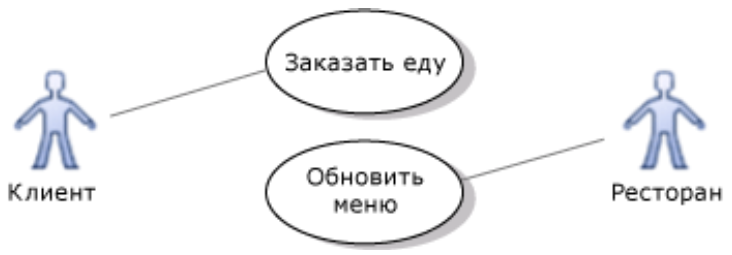
\includegraphics[width=0.5\textwidth]{useCaseSmallExample.png}
\end{center}

Также можно показать, как сценарий использования составляется из более мелких сценариев. Например, заказ продуктов питания --- часть процесса покупки, который также включает оплату и доставку.

Кроме того, на этих диаграммах можно показать, какие сценарии использования включены в область разрабатываемых подсистем. Например, изображенная на рисунке ниже подсистема не входит в состав сценария использования <<Доставка еды>>. Это помогает задать контекст для разработки. Это также можно использовать при обсуждении, что будет включено в последующие релизы. Например, можно обсудить, будет ли компонент <<Оплата еды>> в первоначальном релизе системы функционировать непосредственно между рестораном и клиентом (а не обрабатываться в системе). В этом случае в начальном выпуске можно переместить компонент <<Оплата еды>> за пределы прямоугольника системы Dinner Now.

\begin{center}
    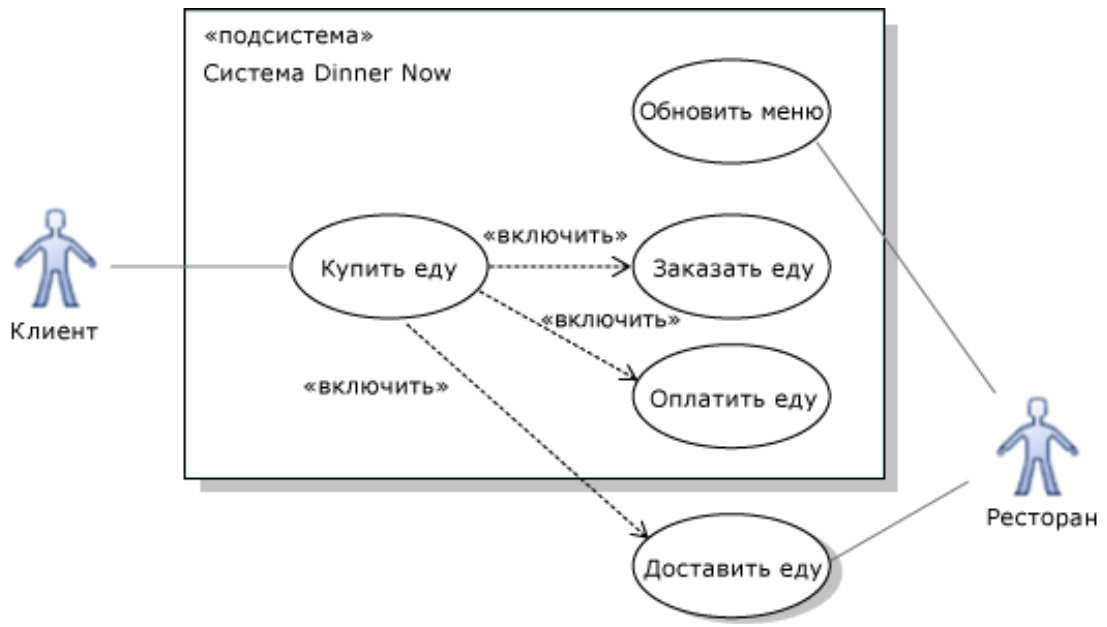
\includegraphics[width=0.5\textwidth]{useCaseBiggerExample.png}
\end{center}

Если число сценариев использования слишком велико, то для упрощения читаемости и поддержки модели целесообразно разделить их по пакетам. Это также упрощает понимание модели и распределение ответственности путем назначения разработчиков, ответственных за пакеты сценариев использования. Пакеты позволяют организовать иерархию требований.

Сценариям могут быть назначены приоритеты: критический, важный и вспомогательный. Критичные сценарии представляют основную системную функциональность или имеют существенное архитектурное значение. Важные сценарии определяют такие системные функции, как сбор статистики, составление отчетов, контроль и функциональное тестирование. Если они не реализованы, то система может выполнять свое предназначение, но со значительно худшим качеством сервиса. Вспомогательные сценарии определяют дополнительную функциональность системы.

Более подробно про синтаксис диаграмм вариантов использования можно почитать, например, в книге Мартина Фаулера <<UML: Основы>>.

Раскрываться сценарии с этих диаграмм могут по-разному, ниже приведён пример формата текстового описания.

\begin{center}
    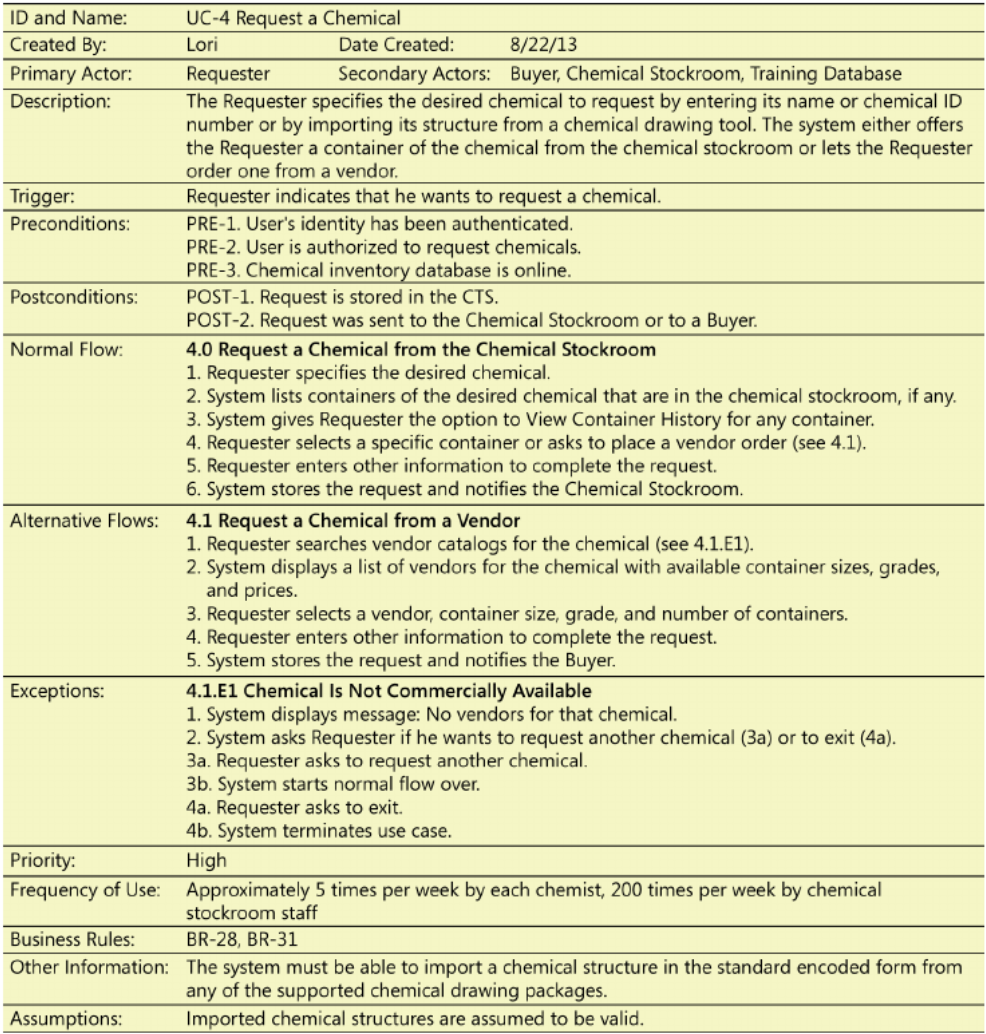
\includegraphics[width=0.9\textwidth]{userScenarioFull.png}
\end{center}

Для более наглядного представления сценариев могут использоваться диаграммы активности UML. Их синтаксис сильно похож на всем известные блок-схемы, и такие диаграммы могут понимать даже самые далёкие от программирования специалисты.

\begin{center}
    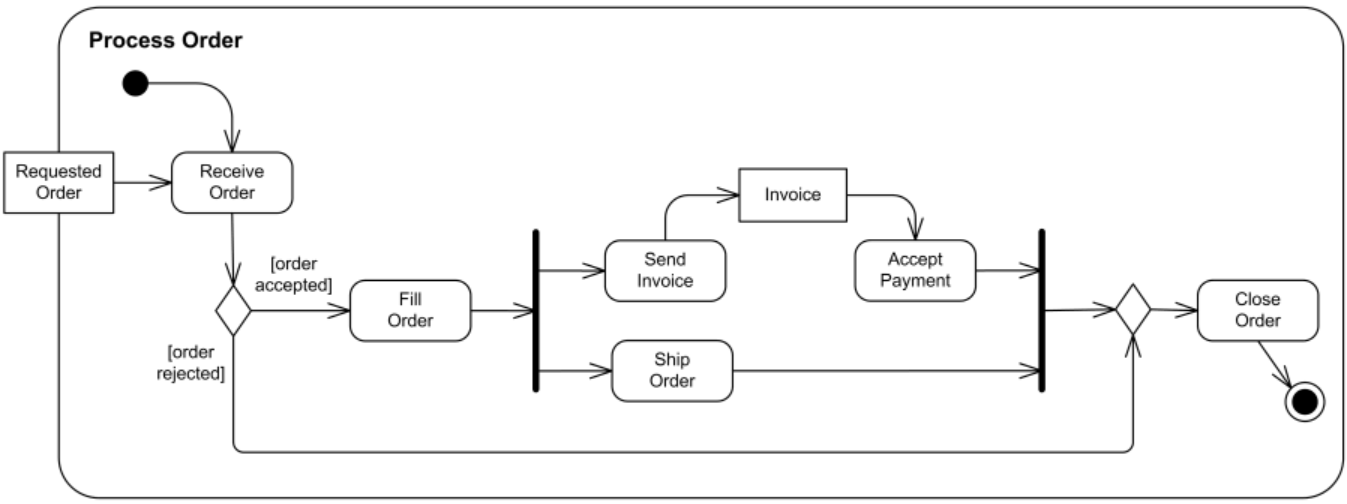
\includegraphics[width=0.9\textwidth]{activity.png}
\end{center}

Если поведение каких-то описываемых объектов лучше всего характеризуется его реакцией на события, произошедшие вне его собственного контекста, то такие объекты называют реактивными. У такого объекта есть четко выраженный жизненный цикл, когда текущее поведение обусловлено прошлым. Например, к этому классу относится подавляющее большинство реальных устройств дискретного управления, другим распространённым примером реактивной системы может служить графический интерфейс пользователя. Для моделирования таких реактивных систем очень хорошо подходят диаграммы конечных автоматов. 

Основными элементами диаграммы конечных автоматов являются <<Состояние>>, <<Событие>> и <<Переход>>. Состояние --- стабильный <<отрезок жизни>> объекта, когда он готов к обработке событий и делает это в зависимости от предыдущей истории поведения. Событие --- происшествие, на которое компонент реагирует и которое может быть создано этим же компонентом (например, компонент посылает сообщение себе самому) или каким-то другим компонентом из окружения. Факт смены одного состояния другим изображается с помощью перехода. Переход осуществляется при наступлении некоторого события.

\begin{center}
    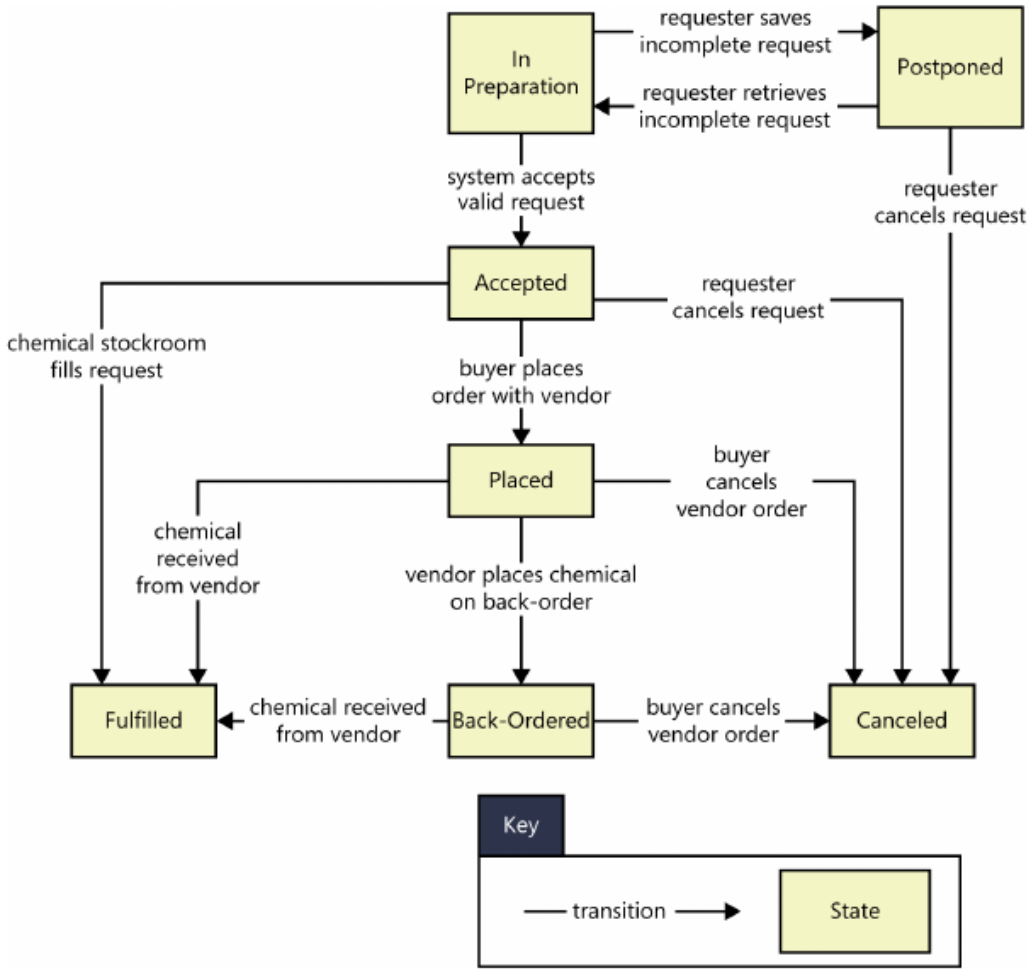
\includegraphics[width=0.9\textwidth]{stateDiagram.png}
\end{center}

Для описания разного рода алгоритмов могут также использоваться деревья или таблицы решений:

\begin{center}
    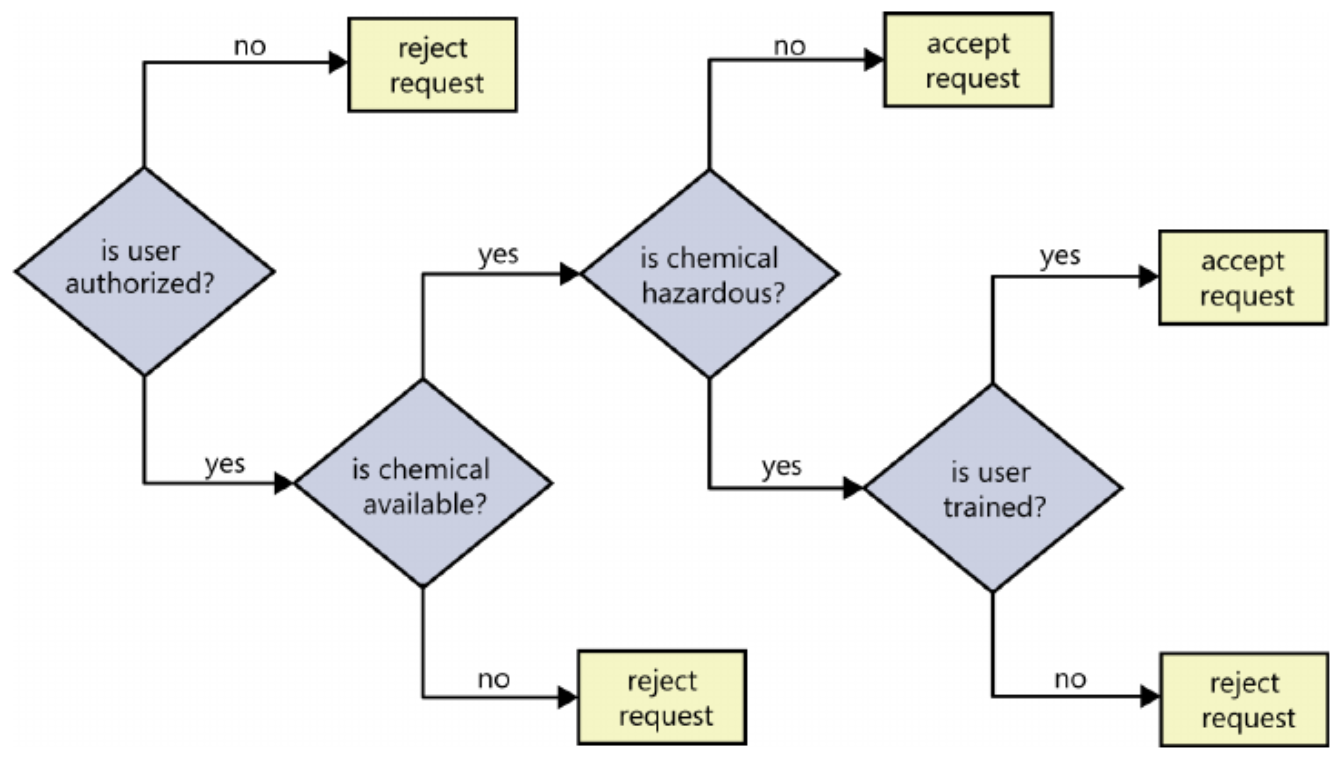
\includegraphics[width=0.9\textwidth]{decisionTrees.png}
\end{center}

\subsection{Спецификация требований к ПО}

На основе созданных моделей и документов часто строится объемлющий документ, содержащий в себе всю собранную информацию. Обычно он прикладывается к договору/контракту или используется как основа для формирования технического задания. Формат такого документа может быть такой:

\begin{enumerate}
    \item Введение
    \begin{enumerate}
        \item Цели
        \item Соглашения о терминах
        \item Предполагаемая аудитория
        \item Масштаб проекта
        \item Ссылки на источники
    \end{enumerate}
    \item Общее описание
    \begin{enumerate}
        \item Видение продукта
        \item Функциональность продукта
        \item Классы и характеристики пользователей
        \item Среда функционирования продукта
        \item Рамки, ограничения, правила и стандарты
        \item Документация для пользователей
        \item Допущения и зависимости
    \end{enumerate}
    \item Функциональность системы
    \begin{enumerate}
        \item Функциональный блок X
        \item Описание и приоритет
        \item Причинно-следственные связи, алгоритмы
        \item Функциональные требования
    \end{enumerate}
    \item Требования к внешним интерфейсам
    \begin{enumerate}
        \item Интерфейсы пользователя (UX)
        \item Программные интерфейсы
        \item Интерфейсы оборудования
        \item Интерфейсы связи и коммуникации
    \end{enumerate}
    \item Нефункциональные требования
    \begin{enumerate}
        \item Требования к производительности
        \item Требования к сохранности (данных)
        \item Критерии качества ПО
        \item Требования к безопасности системы
    \end{enumerate}
    \item Прочие требования
\end{enumerate}

\section{Требования и тестирование}

Требования в явном виде являются источником информации для тестирования системы. На этапе проектирования требования можно использовать для проверки адекватности архитектуры, по ходу разработки требования могут превращаться в приёмочные тесты к системе в целом.

\begin{center}
    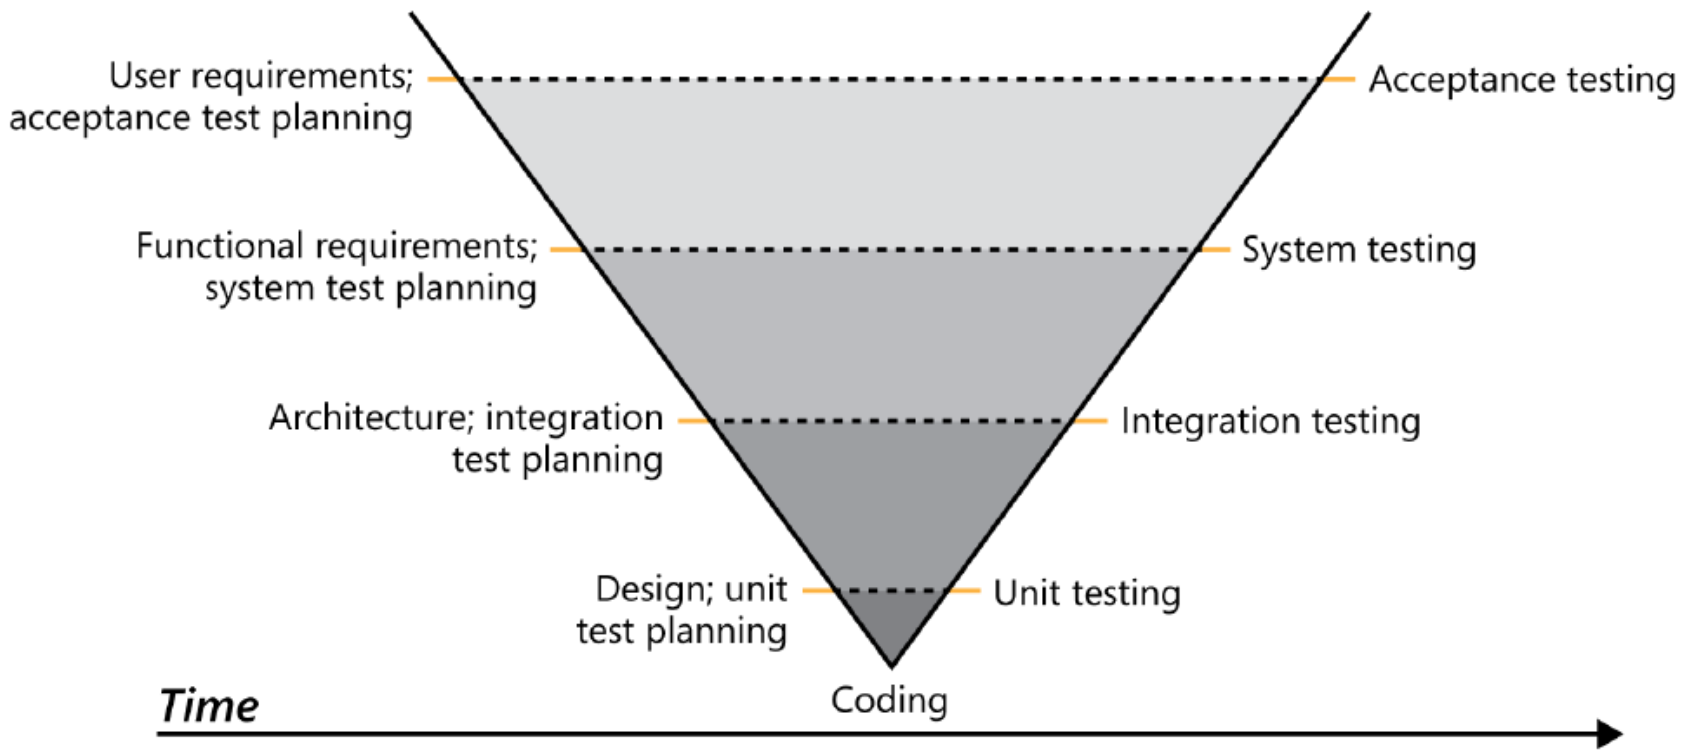
\includegraphics[width=0.9\textwidth]{requirementsAndTesting.png}
\end{center}

\section{Управление требованиями}

Начальные требования неизбежно корректируются в процессе работы клиентами, менеджерами, специалистами по маркетингу, разработчиками и другими лицами. Для эффективного управления требованиями необходим процесс, позволяющий предлагать изменения и оценивать их возможную стоимость и влияние на проект. Контроль за выполнением требований на разных стадиях разработки и тестирования системы позволяет лучше понять состояние проекта в целом. Рассмотрим основные виды деятельности, направленные на управление требованиями во время разработки проекта.

\textbf{Определение процесса управления изменениями.} Определите процесс представления, анализа и утверждения или отклонения изменений к требованиям. Применяйте его для управления всеми предлагаемыми изменениями без исключения. Из представителей заинтересованных в проекте лиц организуйте совет по управлению изменениями, который будет получать информацию о предполагаемых изменениях требований, оценивать ее, решать, какие изменения принять, а какие отклонить, и определять, в какой версии продукта будет внедрена та или иная функция. Даже если этот совет будет состоять из одного человека, важно, чтобы он был, и все изменения проходили через него. Если изменения будут попадать в проект мимо этого совета (например, напрямую от заказчиков к программистам), это по сути сведёт на нет все усилия по планированию и управлению ходом проекта.

\textbf{Создание базовой версии и управление версиями требований.} Базовая версия содержит требования, утвержденные для реализации в конкретной версии продукта. После определения базовых требований изменения можно вносить только в соответствии с процессом управления изменениями. Присвойте всем версиям спецификации требований уникальные идентификаторы, чтобы избежать путаницы между черновыми вариантами и базовыми версиями, а также между предыдущей и текущей версиями требований. Более надежное решение --- управлять версиями документов с требованиями при помощи соответствующих средств управления конфигурацией.

\textbf{Использование средств версионирования и управления требованиями.} Простейший механизм управления версиями --- именовать вручную каждую версию спецификации требований к ПО согласно соглашению. Попытка различать версии документов по дате изменения или дате печати часто приводит к ошибкам и неразберихе, лучше на это не закладываться.

Более сложный метод предполагает сохранение спецификации требований в средстве контроля версий, по аналогии с тем, как версионируется программный код. Хранить файлы в формате Microsoft Word в git’е --- не самое красивое решение, но оно вполне себе работает, и оно гораздо лучше, чем ничего. Наиболее надежный метод контроля версий заключается в хранении требований в базе данных коммерческого средства управления требованиями. Эти средства отслеживают полную историю изменений требований, что особенно важно, если нужно вернуться к более ранней версии требования. Такое средство позволяет вносить комментарии, где можно разумно обосновать решение о добавлении, изменении или удалении требования; эти комментарии могут оказаться полезными при необходимости обсуждения требования в будущем.

Вне зависимости от того, как именно происходит версионирование, для каждого требования полезно указывать следующие атрибуты:
\begin{itemize}
    \item дата создания, автор;
    \item номер текущей ревизии;
    \item лицо, ответственное за удовлетворение требования;
    \item происхождение или источник требования;
    \item состояние (proposed, approved, implemented, verified, rejected и т.п.);
    \item приоритет;
    \item подсистемы, для которых актуально требование;
    \item номер версии продукта, для которой актуально требование;
    \item критерий приемлемости, используемый метод проверки.
\end{itemize}

\textbf{Анализ влияния изменений требований.} Анализ влияния изменений помогает совету по управлению изменениями принимать обоснованные решения. Оцените, как каждое предлагаемое изменение требований повлияет на проект. Выявите другие требования, элементы архитектуры, исходный код и сценарии тестирования, которые, возможно, придется изменить. Определите, что необходимо для реализации изменений, и оцените затраты на peaлизацию.

\textbf{Оценка изменяемости требований.} Регулярно фиксируйте количество требований, внесенных в базовую версию, а также число предложенных и одобренных изменений (добавлений, модификаций и удалений). Если требования формируются не самим клиентом, а от его лица, может оказаться, что проблема понята плохо, границы проекта определены нечетко, бизнес стремительно меняется, при сборе информации многие требования были упущены или внутрикорпоративные политики меняются в худшую сторону.

\section{Литература}

\begin{itemize}
    \item Karl Wiegers. Software Requirements: \url{https://www.amazon.com/Software-Requirements-Developer-Best-Practices/dp/0735679665}
    \item Полезный курс на Степике: \url{https://stepik.org/course/1128}
    \item Блог на тему: \url{http://foranalysts.blogspot.ru/}
\end{itemize}

\end{document}
